\documentclass[../fem.tex]{subfiles}

\begin{document}
\section{Mesh Generation}%
\label{sec:mesh_generation}

For the implementation of FEM, we must discretize our global domain into a set
of finite subdomains, which we call elements. We can then compute our
approximation on each element independent of the rest of the domain, then
combine the solutions of each element into our global solution.

These elements can be of the form of an $N$ sided polygon. However, with
polygons with more than $3$ edges, issues can arise. So for the purposes of
FEM, we will be focused on the construction of a mesh of triangles. This is the
most common mesh polygon, as any mesh of polygons with more edges can be
represented by a triangular mesh. In addition, most research of mesh generation
has been focused on triangular meshes for this same reason.

Our process will be construction what is known as a Constrained Delaunay
Triangulation, and then apply a refinement algorithm to ensure that the
triangles in the mesh are ``nice''.

\subsection{Delaunay Triangulation}%
\label{sub:delaunay_triangulation}

Delaunay triangulation is the straight line dual of the Voronoi diagram.
Delaunay triangulations are used in many different situations, including our
purpose of mesh generation for finite element analysis.

\gtodo{Add example image of Delaunay triangulation.}

A key property of Delaunay triangulation is that no point may lie inside the
circumcircle of any other triangle. We use this as our definition of Delaunay
Triangulation.

\begin{definition}[Delaunay Triangulation] \label{def:dt}
  Let $S$ be a set of points in the plane. A triangulation $T$ is
  a \textit{Delaunay triangulation}($DT$) of $S$ if for each triangle $t$ of $T$
  there exists a circle $C$ with the following properties:
  \begin{enumerate}
    \item the vertices of the triangle $t$ are on the boundary of circle $C$
    \item no other vertex of $S$ is in the interior of $C$.
  \end{enumerate}
\end{definition}

\gtodo{Add image showing circumcircle definition.}
\begin{Figure}
   \begin{center}
     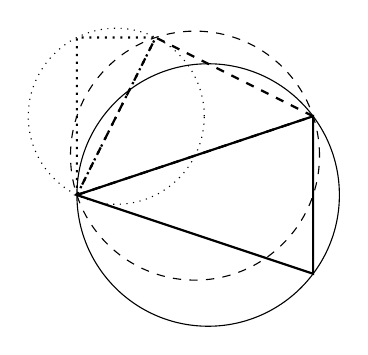
\begin{tikzpicture}
\draw[solid,thick] (0,1) -- (3,0) -- (3,2) -- cycle;
\draw[solid] (1.667, 1) circle (1.66666);
\draw[dashed,thick] (0,1) -- (3,2) -- (1,3) -- cycle;
\draw[dashed] (1.5, 1.5) circle (1.58113);
\draw[dotted,thick] (0,1) -- (1,3) -- (0,3) -- cycle;
\draw[dotted] (0.5,2) circle (1.11803);
\end{tikzpicture}

   \end{center}
   \captionof{figure}{Demonstration of the Circumcircle definition of Delaunay.
   This shows how the circumcircle of each triangle does not contain any vertex
 from any other triangles.}
\end{Figure}

Is most situation the Delaunay triangulation of a set of points is unique. This
is true for all points with one exception of a square, where there are two
valid Delaunay triangulations.

A major advantage of Delaunay triangulation is that it avoids triangles with
small included angles. This makes this type of triangulation extremely well
suited for our purpose of FEA.

There are many different algorithms that can be used for the construction of
Delaunay triangulation of a set of points in a plane. Some notable ones
include; Divide and Conquer developed by Chew\cite{C_CDT}, Incremental
developed by Watson, Sweep Line developed by \v{Z}alik\cite{Z_DT}\cite{DZ_CDT},
and Edge Flipping developed by Sloan\cite{S_DT}\cite{S_CDT}. Each of these
methods has different advantages and different efficiency in computation time.

\subsection{Constrained Delaunay Triangulation}%
\label{sub:constrained_delaunay_triangulation}

The Constrained Delaunay Triangulation(CDT), is a modification of the Delaunay
Triangulation such that specified edges are forced to exist in the
triangulation. This has the unfortunate effect of the resulting triangulation
not being strictly Delaunay. Thus we define our constrained triangulation at
the closest triangulation to the Delaunay triangulation that still includes the
specified edges.

This sence of closeness is such that it is as few modifications from an actual
dalaunay triangulation, that still enforces the constrained edges.

\begin{Figure}
  \begin{center}
    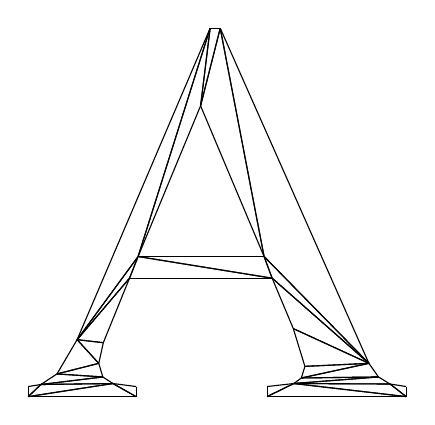
\begin{tikzpicture}[scale=8.0]
\draw (0.2,-0.7924) -- (0.22,-0.7732);
\draw (0.22,-0.7732) -- (0.2,-0.7764);
\draw (0.2,-0.7764) -- (0.2,-0.7924);
\draw (0.22,-0.7732) -- (0.2,-0.7924);
\draw (0.2,-0.7924) -- (0.3344,-0.7716);
\draw (0.3344,-0.7716) -- (0.22,-0.7732);
\draw (0.3712,-0.7924) -- (0.3712,-0.7764);
\draw (0.3712,-0.7764) -- (0.3344,-0.7716);
\draw (0.3344,-0.7716) -- (0.3712,-0.7924);
\draw (0.3344,-0.7716) -- (0.3184,-0.7612);
\draw (0.3184,-0.7612) -- (0.22,-0.7732);
\draw (0.22,-0.7732) -- (0.3344,-0.7716);
\draw (0.3712,-0.7924) -- (0.3344,-0.7716);
\draw (0.3344,-0.7716) -- (0.2,-0.7924);
\draw (0.2,-0.7924) -- (0.3712,-0.7924);
\draw (0.22,-0.7732) -- (0.3184,-0.7612);
\draw (0.3184,-0.7612) -- (0.2456,-0.7564);
\draw (0.2456,-0.7564) -- (0.22,-0.7732);
\draw (0.2456,-0.7564) -- (0.312,-0.7396);
\draw (0.312,-0.7396) -- (0.2776,-0.702);
\draw (0.2776,-0.702) -- (0.2456,-0.7564);
\draw (0.312,-0.7396) -- (0.2456,-0.7564);
\draw (0.2456,-0.7564) -- (0.3184,-0.7612);
\draw (0.3184,-0.7612) -- (0.312,-0.7396);
\draw (0.2776,-0.702) -- (0.312,-0.7396);
\draw (0.312,-0.7396) -- (0.3192,-0.7068);
\draw (0.3192,-0.7068) -- (0.2776,-0.702);
\draw (0.4888,-0.2076) -- (0.2776,-0.702);
\draw (0.2776,-0.702) -- (0.3744,-0.57);
\draw (0.3744,-0.57) -- (0.4888,-0.2076);
\draw (0.3608,-0.6044) -- (0.3744,-0.57);
\draw (0.3744,-0.57) -- (0.2776,-0.702);
\draw (0.2776,-0.702) -- (0.3608,-0.6044);
\draw (0.3744,-0.57) -- (0.3608,-0.6044);
\draw (0.3608,-0.6044) -- (0.5872,-0.6044);
\draw (0.5872,-0.6044) -- (0.3744,-0.57);
\draw (0.3608,-0.6044) -- (0.2776,-0.702);
\draw (0.2776,-0.702) -- (0.3192,-0.7068);
\draw (0.3192,-0.7068) -- (0.3608,-0.6044);
\draw (0.4888,-0.2076) -- (0.3744,-0.57);
\draw (0.3744,-0.57) -- (0.4736,-0.3308);
\draw (0.4736,-0.3308) -- (0.4888,-0.2076);
\draw (0.5792,-0.7924) -- (0.6216,-0.7716);
\draw (0.6216,-0.7716) -- (0.5792,-0.7764);
\draw (0.5792,-0.7764) -- (0.5792,-0.7924);
\draw (0.6216,-0.7716) -- (0.5792,-0.7924);
\draw (0.5792,-0.7924) -- (0.8,-0.7924);
\draw (0.8,-0.7924) -- (0.6216,-0.7716);
\draw (0.8,-0.7924) -- (0.8,-0.7764);
\draw (0.8,-0.7764) -- (0.7744,-0.7724);
\draw (0.7744,-0.7724) -- (0.8,-0.7924);
\draw (0.756,-0.7612) -- (0.6216,-0.7716);
\draw (0.6216,-0.7716) -- (0.7744,-0.7724);
\draw (0.7744,-0.7724) -- (0.756,-0.7612);
\draw (0.756,-0.7612) -- (0.6336,-0.7628);
\draw (0.6336,-0.7628) -- (0.6216,-0.7716);
\draw (0.6216,-0.7716) -- (0.756,-0.7612);
\draw (0.7744,-0.7724) -- (0.6216,-0.7716);
\draw (0.6216,-0.7716) -- (0.8,-0.7924);
\draw (0.8,-0.7924) -- (0.7744,-0.7724);
\draw (0.5048,-0.2076) -- (0.5744,-0.57);
\draw (0.5744,-0.57) -- (0.7408,-0.7396);
\draw (0.7408,-0.7396) -- (0.5048,-0.2076);
\draw (0.3744,-0.57) -- (0.5872,-0.6044);
\draw (0.5872,-0.6044) -- (0.5744,-0.57);
\draw (0.5744,-0.57) -- (0.3744,-0.57);
\draw (0.4888,-0.2076) -- (0.4736,-0.3308);
\draw (0.4736,-0.3308) -- (0.5048,-0.2076);
\draw (0.5048,-0.2076) -- (0.4888,-0.2076);
\draw (0.5744,-0.57) -- (0.5872,-0.6044);
\draw (0.5872,-0.6044) -- (0.7408,-0.7396);
\draw (0.7408,-0.7396) -- (0.5744,-0.57);
\draw (0.4736,-0.3308) -- (0.5744,-0.57);
\draw (0.5744,-0.57) -- (0.5048,-0.2076);
\draw (0.5048,-0.2076) -- (0.4736,-0.3308);
\draw (0.6336,-0.7628) -- (0.7408,-0.7396);
\draw (0.7408,-0.7396) -- (0.6392,-0.7444);
\draw (0.6392,-0.7444) -- (0.6336,-0.7628);
\draw (0.7408,-0.7396) -- (0.6336,-0.7628);
\draw (0.6336,-0.7628) -- (0.756,-0.7612);
\draw (0.756,-0.7612) -- (0.7408,-0.7396);
\draw (0.6208,-0.6844) -- (0.7408,-0.7396);
\draw (0.7408,-0.7396) -- (0.5872,-0.6044);
\draw (0.5872,-0.6044) -- (0.6208,-0.6844);
\draw (0.7408,-0.7396) -- (0.6208,-0.6844);
\draw (0.6208,-0.6844) -- (0.6392,-0.7444);
\draw (0.6392,-0.7444) -- (0.7408,-0.7396);
\end{tikzpicture}

  \end{center}
  \captionof{figure}{Constraied Delaunay triangulation. Of the letter $A$. This
  mesh has been constructed without any quality or refinement.}
\end{Figure}

The constrained edges are most commonly arise for the purpose of defining
boundaries of the domain or enforcing a medium change. This makes it necessary
for any desired domain without a strictly convex outer hull that is generated
from the unconstrained triangulation.

There are several different methods of construction the CDT. A few of these
generate enforce the constraints during the initial construction of the
Delaunay triangulation. However, many more use a preconstructed Delaunay
triangulation and then proceed to enforce the edges, and refactor the mesh
around the forced edge.

\subsection{Edge Flipping}%
\label{sub:edge_flipping}

We utilize an implementation of edge flipping algorithms developed by Sloan.
Sloan's edge flipping algorithm has implementation specifics for both
constrained and unconstrained Delaunay triangulation.

We will provide a short explanation of the method that is used for the
construction of our triangular mesh, but more detail can be found in
\cite{S_DT}\cite{S_CDT}. First Sloan's algorithm constructions the
unconstrained Delaunay triangulation then enforces the required edges into the
triangulation. So, we begin with the process for construction the unconstrained
triangulations.

\subsubsection{Construction of Delaunay Triangulation}%
\label{ssub:construction_of_delaunay_triangulation}

Using this method also provides the advantage of generating a triangle
adjacency list for each of the triangles. This allows for optimizations later
in the process of finite element analysis.

There are seven main stages of the construction of the Delaunay triangulation.
We also define $G$ as the set of points to be triangulated, and $N$ as the
number of points in $G$.

\begin{enumerate}[label=\arabic*.]
  \item Normalize coordinates of points.
  \item Sort points into bins.
  \item Establish the super triangle.
  \item Loop over each point, repeating 5-7
  \item Insert new point in triangulation.
  \item Initialize stack.
  \item Restore Delaunay triangulation.
\end{enumerate}

In stage 1, we scale all the points that will be used to construct the
triangulation between $0$ and $1$, this should be done such that all relative
positions of points are unchanged. This is done using
\begin{align*}
  \hat{x}=\frac{x-x_{min}}{d_{max}},\quad\hat{y}=\frac{y-y_{min}}{d_{max}},
\end{align*}
where
\begin{align*}
  d_{max}=\max\left\{x_{max}-x_{min},\ y_{max}-y_{min}\right\}.
\end{align*}
This will scale all coordinates between $0$ and $1$ but will maintain the
relative positions to all other points.

In stage 2, the normalized points are sorted into a set of bins. Each bin is
associated with a rectangular portion of global space that the points are
included in. We construction the bins such that each bin contains roughly
$\sqrt{N}$ points. The bins are then ordered such that adjacent bins are
numbered consecutively. This is done to improve the efficiency of later
searching of the triangular mesh.

In step 3, we construction a ``super triangle''. This triangle is a triangle of
three additional points, such that all points in $G$ are enclosed within the
super triangle.

In stage 4, we repeat stages 5-7 for every $P$ in $G$.

In step 5, we determine the triangle which encloses $P$(Since the super
triangle encloses all points, then this triangle must exist for $P$). We now
delete this triangle, and construct three new triangles, by connection $P$ to
the three vertices of the deleted triangle.

In step 6, we add up to three triangles that are adjacent to the edges opposite
$P$ to a stack(A \textit{stack} is a last in first out data structure, like a
stack of trays).

In step 7, while the stack is not empty we proceed as following

\begin{enumerate}[label=7.\arabic*.]
  \item Remove triangle from top of the stack.
  \item If $P$ is within the circumcircle of this triangle, then the adjacent
    triangle containing $P$ and the unstacked triangle form a convex
    quadrilateral whose diagonal is drawn in the non-optimal direction. Swap
    this diagonal edge.
  \item Add any new triangles which are opposite $P$ to the stack.
\end{enumerate}

After the stack is empty, then Delaunay triangulation has been restored.

Once every point has been added to the triangulation, then the completed
Delaunay triangulation can be returned.

\subsubsection{Construction of Constrained Delaunay Triangulation}%
\label{ssub:construction_of_constrained_delaunay_triangulation}

Now that a Delaunay triangulation has been constructed for our set of $G$
points, we now modify the triangulation so to ensure that certain edges are
present.

This process proceeds as follows

\begin{enumerate}[label=\arabic*.]
  \item Loop over each constrained edge.
  \item Find intersecting edges.
  \item Remove intersecting edges.
  \item Restore Delaunay triangulation.
  \item Remove superfluous triangles.
\end{enumerate}

In step 1, we loop over every edge to be constrained, and we define the edge by
the endpoints of the edge $V_i$ and $V_j$. Using this edge repeat steps 2-4.

In stage 2, we find all edges in the triangulation that intersect $V_i-V_j$.
Store all of these edges in a list. If our constrained edge is already present
in the triangulation, the go to step 1.

In step 3, repeat while there are still edges that intersect $V_i-V_j$.
\begin{enumerate}[label=3.\arabic*.]
  \item Remove an edge from the list of intersecting edges, call this edge
    $V_k-V_l$.
  \item If the triangles that share the edge $V_k-V_l$ do not form a strictly
    convex quadrilateral, then place the edge back on the list of edges and go
    to step 3. Else, swap this diagonal, and define the new diagonal as
    $V_m-V_n$. If $V_m-V_n$ still intersections $V_i-V_j$, then place it back
    on the list of new edges, otherwise place $V_m-V_n$ on a list of new edges.
\end{enumerate}

In step 4, repeat until no changes occur.
\begin{enumerate}[label=4.\arabic*.]
  \item Loop over each newly created edge, define each edge by $V_k-V_l$.
  \item If $V_k-V_l$ is equal to $V_i-V_j$, then skip to step $4.1$.
  \item If the two triangles that share the edge $V_k-V_l$ do not satisfy the
    Delaunay criterion, then swap the diagonal, and place the new diagonal on
    the list of new edges.
\end{enumerate}

In step 5, we need to remove all unwanted triangles. For this stage, we differ
from the process of Sloan. This is because for our implementation we desire the
ability to have holes in the mesh, and the simplistic method of removing
exterior triangles will not achieve this.

We use what is known as a triangle infection algorithm. Where we define a few
points that will infect the triangles which the points are within, then the
infection spreads to all adjacent triangles that are not separated by a
constrained edge. This process is repeated until no new triangles become
infected. Then all infected triangles are removed.

With this process, we need to define a point that is within every one of the
holes in the mesh, as the initial infection point, then the three vertices of
the super triangle are also used as initial infection points.

After all infected triangles are removed, we have constructed our constrained
Delaunay triangulation, which can then be used for FEA.

\subsection{Mesh Refinement}%
\label{sub:mesh_refinement}

The raw result of our constrained Delaunay triangulation algorithm may be
sufficient in a few situations, but for most purposes, it returns sub-optimal
meshes. Because of this, we must implement a mesh refinement algorithm to
improve upon the quality of our mesh.

There are two main mesh refinement algorithms, Ruppert's algorithm
\cite{R_REF}, and Chew's second algorithm \cite{C_REF}. These two algorithms
work with a similar principle, but we will focus on Chew's second algorithm. We
do this because of the advantages that Chew's second algorithm provides over
Ruppert's.

Mesh refinement is required because triangular elements along constrained
edges are currently forced to have the constrained edge and one of their edges.
This can cause these triangles to be skinny sliver triangles, ones that are
undesirable in our final mesh. To fix this we define a notion of ``nice''
triangles, and insert new points into the mesh until all triangles satisfy
our definition of ``nice''.

\begin{definition}[Well-shaped]\label{def:well_shaped_tri}
  A triangle is well-shaped if all its angles are greater than or equal to some
  angle $\alpha$ (commonly $\alpha=30^{\circ}$).
\end{definition}

\begin{definition}[Well-sized]\label{def:well_sized_tri}
  A triangle is well-sized if the area of the triangle satisfies some user
  defined grading function $g$ (commonly $g=\text{const}$). This function can
  use any criteria as long as there exists a value $\delta > 0$ such that any
  well-shaped(Def \ref{def:well_shaped_tri}) triangle that fits within a circle
  of radius $\delta$ would satisfy the grading function.
\end{definition}

\begin{definition}[\textit{Nice} Triangle] \label{def:nice_tri}
  A triangle is \textit{nice} if it is both well-shaped(Def
  \ref{def:well_shaped_tri}) and well-sized(Def \ref{def:well_sized_tri}).
\end{definition}

The use of a non-constant grading function is to allow dynamically sized
meshes.  Such that in areas of interest there can be significantly more
refinement, and areas of less interest can be generalized. The restrictions on
the function simply stated is that there must be some size of a triangle that
will satisfy the grading function everywhere, and that the grading function
does not get infinitely strict at any point.

Using these definitions we are able to implement the mesh refinement algorithm.
Chew's second algorithm proceeds as follows.

\begin{enumerate}[label=\arabic*.]
  \item Grade any triangles that are currently ungraded. A triangle only passes
    if it is \textit{nice}(Def \ref{def:nice_tri}).
  \item If all triangles pass then Halt. Otherwise select the larges triangle
    that fails $\Delta$, and determine its circumcenter $c$.
  \item Traverse the triangulation from any vertex of $\Delta$ in the direction
    of $c$ until either running into a source-edge or finding the triangle
    containing $c$.
  \item If the triangle containing $c$ was found then insert $c$ into the
    triangulation, and update the triangulation to be Delaunay. This process is
    similar to that of sec \ref{sub:edge_flipping}. Then go to step 2.
  \item If a source edge was encountered, then split the source edge into two
    equal sized edges and update the triangulation. Let $l$ be the length of
    the new edges. Delete each circumcenter-vertex(vertices that are not part
    of the original triangulation) that is within $l$(line-of-sight distance,
    where a source-edge means that a vertex is infinitely far away) of the new
    vertex. Then go to step 2.
\end{enumerate}

Using this algorithm it is possible to construct triangulations with a required
minimum angle and force a size function. This provides the ability of
guaranteed \textit{nice} triangular meshes for any desired input domain.

Both Chew's second algorithm and Ruppert's algorithm have proven termination
for minimum angles below a certain point. For Rupert's algorithm, any minimum
angle below $20.7^{\circ}$ is guaranteed to halt. While Chew's second algorithm
is guaranteed to halt for angles below $28.6^{\circ}$ and will often succeed
with angles below $34^{\circ}$. Because of this improvement on the guaranteed
minimum angle is why our focus is on Chew's algorithm for mesh refinement.

\begin{Figure}
   \begin{center}
     \begin{minipage}{0.4\textwidth}
       \begin{center}
         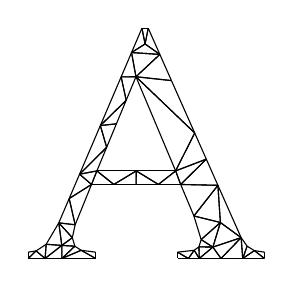
\begin{tikzpicture}[scale=5]
\draw (0.2,-0.7924) -- (0.22,-0.7732);
\draw (0.22,-0.7732) -- (0.2,-0.7764);
\draw (0.2,-0.7764) -- (0.2,-0.7924);
\draw (0.28531162790697684,-0.7592558139534884) -- (0.2428,-0.7924);
\draw (0.2428,-0.7924) -- (0.28559999999999997,-0.7924);
\draw (0.28559999999999997,-0.7924) -- (0.28531162790697684,-0.7592558139534884);
\draw (0.4736,-0.3308) -- (0.5343,-0.2741);
\draw (0.5343,-0.2741) -- (0.46240000000000003,-0.2694);
\draw (0.46240000000000003,-0.2694) -- (0.4736,-0.3308);
\draw (0.4174,-0.6044) -- (0.47400000000000003,-0.6044);
\draw (0.47400000000000003,-0.6044) -- (0.47440000000000004,-0.57);
\draw (0.47440000000000004,-0.57) -- (0.4174,-0.6044);
\draw (0.3712,-0.7924) -- (0.3712,-0.7764);
\draw (0.3712,-0.7764) -- (0.3344,-0.7716);
\draw (0.3344,-0.7716) -- (0.3712,-0.7924);
\draw (0.6216,-0.7716) -- (0.6068,-0.7924);
\draw (0.6068,-0.7924) -- (0.6344000000000001,-0.7924);
\draw (0.6344000000000001,-0.7924) -- (0.6216,-0.7716);
\draw (0.436,-0.3312) -- (0.44880000000000003,-0.39059999999999995);
\draw (0.44880000000000003,-0.39059999999999995) -- (0.4736,-0.3308);
\draw (0.4736,-0.3308) -- (0.436,-0.3312);
\draw (0.3184,-0.7612) -- (0.312,-0.7396);
\draw (0.312,-0.7396) -- (0.28531162790697684,-0.7592558139534884);
\draw (0.28531162790697684,-0.7592558139534884) -- (0.3184,-0.7612);
\draw (0.28559999999999997,-0.7924) -- (0.3344,-0.7716);
\draw (0.3344,-0.7716) -- (0.3184,-0.7612);
\draw (0.3184,-0.7612) -- (0.28559999999999997,-0.7924);
\draw (0.3712,-0.7924) -- (0.3344,-0.7716);
\draw (0.3344,-0.7716) -- (0.28559999999999997,-0.7924);
\draw (0.28559999999999997,-0.7924) -- (0.3712,-0.7924);
\draw (0.3744,-0.57) -- (0.3608,-0.6044);
\draw (0.3608,-0.6044) -- (0.4174,-0.6044);
\draw (0.4174,-0.6044) -- (0.3744,-0.57);
\draw (0.2456,-0.7564) -- (0.22,-0.7732);
\draw (0.22,-0.7732) -- (0.2428,-0.7924);
\draw (0.2428,-0.7924) -- (0.2456,-0.7564);
\draw (0.28531162790697684,-0.7592558139534884) -- (0.2776,-0.702);
\draw (0.2776,-0.702) -- (0.2456,-0.7564);
\draw (0.2456,-0.7564) -- (0.28531162790697684,-0.7592558139534884);
\draw (0.28559999999999997,-0.7924) -- (0.3184,-0.7612);
\draw (0.3184,-0.7612) -- (0.28531162790697684,-0.7592558139534884);
\draw (0.28531162790697684,-0.7592558139534884) -- (0.28559999999999997,-0.7924);
\draw (0.2776,-0.702) -- (0.312,-0.7396);
\draw (0.312,-0.7396) -- (0.3192,-0.7068);
\draw (0.3192,-0.7068) -- (0.2776,-0.702);
\draw (0.3192,-0.7068) -- (0.304,-0.6402);
\draw (0.304,-0.6402) -- (0.2776,-0.702);
\draw (0.2776,-0.702) -- (0.3192,-0.7068);
\draw (0.3744,-0.57) -- (0.33039999999999997,-0.5784);
\draw (0.33039999999999997,-0.5784) -- (0.3608,-0.6044);
\draw (0.3608,-0.6044) -- (0.3744,-0.57);
\draw (0.6208,-0.6844) -- (0.6818,-0.6066);
\draw (0.6818,-0.6066) -- (0.5872,-0.6044);
\draw (0.5872,-0.6044) -- (0.6208,-0.6844);
\draw (0.3992,-0.5102) -- (0.33039999999999997,-0.5784);
\draw (0.33039999999999997,-0.5784) -- (0.3744,-0.57);
\draw (0.3744,-0.57) -- (0.3992,-0.5102);
\draw (0.5306000000000001,-0.6044) -- (0.5872,-0.6044);
\draw (0.5872,-0.6044) -- (0.5744,-0.57);
\draw (0.5744,-0.57) -- (0.5306000000000001,-0.6044);
\draw (0.304,-0.6402) -- (0.3192,-0.7068);
\draw (0.3192,-0.7068) -- (0.3608,-0.6044);
\draw (0.3608,-0.6044) -- (0.304,-0.6402);
\draw (0.2776,-0.702) -- (0.28531162790697684,-0.7592558139534884);
\draw (0.28531162790697684,-0.7592558139534884) -- (0.312,-0.7396);
\draw (0.312,-0.7396) -- (0.2776,-0.702);
\draw (0.6880643863623271,-0.7010295113359224) -- (0.6690356340288925,-0.7635325842696628);
\draw (0.6690356340288925,-0.7635325842696628) -- (0.7408,-0.7396);
\draw (0.7408,-0.7396) -- (0.6880643863623271,-0.7010295113359224);
\draw (0.22,-0.7732) -- (0.2,-0.7924);
\draw (0.2,-0.7924) -- (0.2428,-0.7924);
\draw (0.2428,-0.7924) -- (0.22,-0.7732);
\draw (0.44880000000000003,-0.39059999999999995) -- (0.3832,-0.4548);
\draw (0.3832,-0.4548) -- (0.42400000000000004,-0.45039999999999997);
\draw (0.42400000000000004,-0.45039999999999997) -- (0.44880000000000003,-0.39059999999999995);
\draw (0.6068,-0.7924) -- (0.5792,-0.7764);
\draw (0.5792,-0.7764) -- (0.5792,-0.7924);
\draw (0.5792,-0.7924) -- (0.6068,-0.7924);
\draw (0.7448,-0.7924) -- (0.8,-0.7924);
\draw (0.8,-0.7924) -- (0.7744,-0.7724);
\draw (0.7744,-0.7724) -- (0.7448,-0.7924);
\draw (0.3832,-0.4548) -- (0.3992,-0.5102);
\draw (0.3992,-0.5102) -- (0.42400000000000004,-0.45039999999999997);
\draw (0.42400000000000004,-0.45039999999999997) -- (0.3832,-0.4548);
\draw (0.4736,-0.3308) -- (0.6228,-0.4736);
\draw (0.6228,-0.4736) -- (0.5638000000000001,-0.3406);
\draw (0.5638000000000001,-0.3406) -- (0.4736,-0.3308);
\draw (0.8,-0.7924) -- (0.8,-0.7764);
\draw (0.8,-0.7764) -- (0.7744,-0.7724);
\draw (0.7744,-0.7724) -- (0.8,-0.7924);
\draw (0.6523,-0.5401) -- (0.6228,-0.4736);
\draw (0.6228,-0.4736) -- (0.5744,-0.57);
\draw (0.5744,-0.57) -- (0.6523,-0.5401);
\draw (0.7408,-0.7396) -- (0.6896,-0.7924);
\draw (0.6896,-0.7924) -- (0.7448,-0.7924);
\draw (0.7448,-0.7924) -- (0.7408,-0.7396);
\draw (0.6216,-0.7716) -- (0.6344000000000001,-0.7924);
\draw (0.6344000000000001,-0.7924) -- (0.6336,-0.7628);
\draw (0.6336,-0.7628) -- (0.6216,-0.7716);
\draw (0.756,-0.7612) -- (0.7448,-0.7924);
\draw (0.7448,-0.7924) -- (0.7744,-0.7724);
\draw (0.7744,-0.7724) -- (0.756,-0.7612);
\draw (0.756,-0.7612) -- (0.7408,-0.7396);
\draw (0.7408,-0.7396) -- (0.7448,-0.7924);
\draw (0.7448,-0.7924) -- (0.756,-0.7612);
\draw (0.5872,-0.6044) -- (0.6523,-0.5401);
\draw (0.6523,-0.5401) -- (0.5744,-0.57);
\draw (0.5744,-0.57) -- (0.5872,-0.6044);
\draw (0.6896,-0.7924) -- (0.6690356340288925,-0.7635325842696628);
\draw (0.6690356340288925,-0.7635325842696628) -- (0.6344000000000001,-0.7924);
\draw (0.6344000000000001,-0.7924) -- (0.6896,-0.7924);
\draw (0.5343,-0.2741) -- (0.4736,-0.3308);
\draw (0.4736,-0.3308) -- (0.5638000000000001,-0.3406);
\draw (0.5638000000000001,-0.3406) -- (0.5343,-0.2741);
\draw (0.47440000000000004,-0.57) -- (0.3744,-0.57);
\draw (0.3744,-0.57) -- (0.4174,-0.6044);
\draw (0.4174,-0.6044) -- (0.47440000000000004,-0.57);
\draw (0.7408,-0.7396) -- (0.6818,-0.6066);
\draw (0.6818,-0.6066) -- (0.6880643863623271,-0.7010295113359224);
\draw (0.6880643863623271,-0.7010295113359224) -- (0.7408,-0.7396);
\draw (0.4736,-0.3308) -- (0.46240000000000003,-0.2694);
\draw (0.46240000000000003,-0.2694) -- (0.436,-0.3312);
\draw (0.436,-0.3312) -- (0.4736,-0.3308);
\draw (0.5872,-0.6044) -- (0.6818,-0.6066);
\draw (0.6818,-0.6066) -- (0.6523,-0.5401);
\draw (0.6523,-0.5401) -- (0.5872,-0.6044);
\draw (0.5744,-0.57) -- (0.6228,-0.4736);
\draw (0.6228,-0.4736) -- (0.4736,-0.3308);
\draw (0.4736,-0.3308) -- (0.5744,-0.57);
\draw (0.6336,-0.7628) -- (0.6344000000000001,-0.7924);
\draw (0.6344000000000001,-0.7924) -- (0.6690356340288925,-0.7635325842696628);
\draw (0.6690356340288925,-0.7635325842696628) -- (0.6336,-0.7628);
\draw (0.6690356340288925,-0.7635325842696628) -- (0.6392,-0.7444);
\draw (0.6392,-0.7444) -- (0.6336,-0.7628);
\draw (0.6336,-0.7628) -- (0.6690356340288925,-0.7635325842696628);
\draw (0.6880643863623271,-0.7010295113359224) -- (0.6208,-0.6844);
\draw (0.6208,-0.6844) -- (0.6392,-0.7444);
\draw (0.6392,-0.7444) -- (0.6880643863623271,-0.7010295113359224);
\draw (0.6392,-0.7444) -- (0.6690356340288925,-0.7635325842696628);
\draw (0.6690356340288925,-0.7635325842696628) -- (0.6880643863623271,-0.7010295113359224);
\draw (0.6880643863623271,-0.7010295113359224) -- (0.6392,-0.7444);
\draw (0.5792,-0.7764) -- (0.6068,-0.7924);
\draw (0.6068,-0.7924) -- (0.6216,-0.7716);
\draw (0.6216,-0.7716) -- (0.5792,-0.7764);
\draw (0.4968,-0.24755631067961165) -- (0.4888,-0.2076);
\draw (0.4888,-0.2076) -- (0.46240000000000003,-0.2694);
\draw (0.46240000000000003,-0.2694) -- (0.4968,-0.24755631067961165);
\draw (0.46240000000000003,-0.2694) -- (0.5343,-0.2741);
\draw (0.5343,-0.2741) -- (0.4968,-0.24755631067961165);
\draw (0.4968,-0.24755631067961165) -- (0.46240000000000003,-0.2694);
\draw (0.2428,-0.7924) -- (0.28531162790697684,-0.7592558139534884);
\draw (0.28531162790697684,-0.7592558139534884) -- (0.2456,-0.7564);
\draw (0.2456,-0.7564) -- (0.2428,-0.7924);
\draw (0.6818,-0.6066) -- (0.6208,-0.6844);
\draw (0.6208,-0.6844) -- (0.6880643863623271,-0.7010295113359224);
\draw (0.6880643863623271,-0.7010295113359224) -- (0.6818,-0.6066);
\draw (0.6896,-0.7924) -- (0.7408,-0.7396);
\draw (0.7408,-0.7396) -- (0.6690356340288925,-0.7635325842696628);
\draw (0.6690356340288925,-0.7635325842696628) -- (0.6896,-0.7924);
\draw (0.47440000000000004,-0.57) -- (0.5306000000000001,-0.6044);
\draw (0.5306000000000001,-0.6044) -- (0.5744,-0.57);
\draw (0.5744,-0.57) -- (0.47440000000000004,-0.57);
\draw (0.5306000000000001,-0.6044) -- (0.47440000000000004,-0.57);
\draw (0.47440000000000004,-0.57) -- (0.47400000000000003,-0.6044);
\draw (0.47400000000000003,-0.6044) -- (0.5306000000000001,-0.6044);
\draw (0.3832,-0.4548) -- (0.44880000000000003,-0.39059999999999995);
\draw (0.44880000000000003,-0.39059999999999995) -- (0.436,-0.3312);
\draw (0.436,-0.3312) -- (0.3832,-0.4548);
\draw (0.3608,-0.6044) -- (0.33039999999999997,-0.5784);
\draw (0.33039999999999997,-0.5784) -- (0.304,-0.6402);
\draw (0.304,-0.6402) -- (0.3608,-0.6044);
\draw (0.33039999999999997,-0.5784) -- (0.3992,-0.5102);
\draw (0.3992,-0.5102) -- (0.3832,-0.4548);
\draw (0.3832,-0.4548) -- (0.33039999999999997,-0.5784);
\draw (0.5048,-0.2076) -- (0.4888,-0.2076);
\draw (0.4888,-0.2076) -- (0.4968,-0.24755631067961165);
\draw (0.4968,-0.24755631067961165) -- (0.5048,-0.2076);
\draw (0.5343,-0.2741) -- (0.5048,-0.2076);
\draw (0.5048,-0.2076) -- (0.4968,-0.24755631067961165);
\draw (0.4968,-0.24755631067961165) -- (0.5343,-0.2741);
\end{tikzpicture}

         (a)
       \end{center}
     \end{minipage}
     \begin{minipage}{0.4\textwidth}
       \begin{center}
         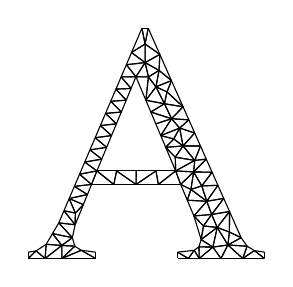
\begin{tikzpicture}[scale=5]
\draw (0.2,-0.7924) -- (0.22,-0.7732);
\draw (0.22,-0.7732) -- (0.2,-0.7764);
\draw (0.2,-0.7764) -- (0.2,-0.7924);
\draw (0.28531162790697684,-0.7592558139534884) -- (0.2428,-0.7924);
\draw (0.2428,-0.7924) -- (0.28559999999999997,-0.7924);
\draw (0.28559999999999997,-0.7924) -- (0.28531162790697684,-0.7592558139534884);
\draw (0.4968406949074053,-0.2948391566292681) -- (0.46240000000000003,-0.2694);
\draw (0.46240000000000003,-0.2694) -- (0.4492,-0.3003);
\draw (0.4492,-0.3003) -- (0.4968406949074053,-0.2948391566292681);
\draw (0.47400000000000003,-0.6044) -- (0.47440000000000004,-0.57);
\draw (0.47440000000000004,-0.57) -- (0.4244,-0.57);
\draw (0.4244,-0.57) -- (0.47400000000000003,-0.6044);
\draw (0.3712,-0.7924) -- (0.3712,-0.7764);
\draw (0.3712,-0.7764) -- (0.3344,-0.7716);
\draw (0.3344,-0.7716) -- (0.3712,-0.7924);
\draw (0.6216,-0.7716) -- (0.6068,-0.7924);
\draw (0.6068,-0.7924) -- (0.6344000000000001,-0.7924);
\draw (0.6344000000000001,-0.7924) -- (0.6216,-0.7716);
\draw (0.436,-0.3312) -- (0.46120000000000005,-0.36069999999999997);
\draw (0.46120000000000005,-0.36069999999999997) -- (0.4736,-0.3308);
\draw (0.4736,-0.3308) -- (0.436,-0.3312);
\draw (0.3184,-0.7612) -- (0.312,-0.7396);
\draw (0.312,-0.7396) -- (0.28531162790697684,-0.7592558139534884);
\draw (0.28531162790697684,-0.7592558139534884) -- (0.3184,-0.7612);
\draw (0.28559999999999997,-0.7924) -- (0.3344,-0.7716);
\draw (0.3344,-0.7716) -- (0.3184,-0.7612);
\draw (0.3184,-0.7612) -- (0.28559999999999997,-0.7924);
\draw (0.3712,-0.7924) -- (0.3344,-0.7716);
\draw (0.3344,-0.7716) -- (0.28559999999999997,-0.7924);
\draw (0.28559999999999997,-0.7924) -- (0.3712,-0.7924);
\draw (0.3744,-0.57) -- (0.3608,-0.6044);
\draw (0.3608,-0.6044) -- (0.4174,-0.6044);
\draw (0.4174,-0.6044) -- (0.3744,-0.57);
\draw (0.2456,-0.7564) -- (0.22,-0.7732);
\draw (0.22,-0.7732) -- (0.2428,-0.7924);
\draw (0.2428,-0.7924) -- (0.2456,-0.7564);
\draw (0.28531162790697684,-0.7592558139534884) -- (0.2616,-0.7292);
\draw (0.2616,-0.7292) -- (0.2456,-0.7564);
\draw (0.2456,-0.7564) -- (0.28531162790697684,-0.7592558139534884);
\draw (0.28559999999999997,-0.7924) -- (0.3184,-0.7612);
\draw (0.3184,-0.7612) -- (0.28531162790697684,-0.7592558139534884);
\draw (0.28531162790697684,-0.7592558139534884) -- (0.28559999999999997,-0.7924);
\draw (0.2776,-0.702) -- (0.312,-0.7396);
\draw (0.312,-0.7396) -- (0.3192,-0.7068);
\draw (0.3192,-0.7068) -- (0.2776,-0.702);
\draw (0.3192,-0.7068) -- (0.2908,-0.6711);
\draw (0.2908,-0.6711) -- (0.2776,-0.702);
\draw (0.2776,-0.702) -- (0.3192,-0.7068);
\draw (0.3744,-0.57) -- (0.33039999999999997,-0.5784);
\draw (0.33039999999999997,-0.5784) -- (0.3608,-0.6044);
\draw (0.3608,-0.6044) -- (0.3744,-0.57);
\draw (0.6208,-0.6844) -- (0.6450980210406373,-0.7097699402142046);
\draw (0.6450980210406373,-0.7097699402142046) -- (0.6659339941556301,-0.6806873886526693);
\draw (0.6659339941556301,-0.6806873886526693) -- (0.6208,-0.6844);
\draw (0.6392,-0.7444) -- (0.6800202045062519,-0.713573727137458);
\draw (0.6800202045062519,-0.713573727137458) -- (0.6450980210406373,-0.7097699402142046);
\draw (0.6450980210406373,-0.7097699402142046) -- (0.6392,-0.7444);
\draw (0.3568,-0.5166) -- (0.3868,-0.5401);
\draw (0.3868,-0.5401) -- (0.3992,-0.5102);
\draw (0.3992,-0.5102) -- (0.3568,-0.5166);
\draw (0.5306000000000001,-0.6044) -- (0.5872,-0.6044);
\draw (0.5872,-0.6044) -- (0.5744,-0.57);
\draw (0.5744,-0.57) -- (0.5306000000000001,-0.6044);
\draw (0.35040000000000004,-0.63) -- (0.3608,-0.6044);
\draw (0.3608,-0.6044) -- (0.3172,-0.6093);
\draw (0.3172,-0.6093) -- (0.35040000000000004,-0.63);
\draw (0.2616,-0.7292) -- (0.312,-0.7396);
\draw (0.312,-0.7396) -- (0.2776,-0.702);
\draw (0.2776,-0.702) -- (0.2616,-0.7292);
\draw (0.7109619922876913,-0.7252980211896037) -- (0.6800202045062519,-0.713573727137458);
\draw (0.6800202045062519,-0.713573727137458) -- (0.7071175748135642,-0.7581624967889107);
\draw (0.7071175748135642,-0.7581624967889107) -- (0.7109619922876913,-0.7252980211896037);
\draw (0.22,-0.7732) -- (0.2,-0.7924);
\draw (0.2,-0.7924) -- (0.2428,-0.7924);
\draw (0.2428,-0.7924) -- (0.22,-0.7732);
\draw (0.40959999999999996,-0.393) -- (0.4364,-0.4205);
\draw (0.4364,-0.4205) -- (0.44880000000000003,-0.39059999999999995);
\draw (0.44880000000000003,-0.39059999999999995) -- (0.40959999999999996,-0.393);
\draw (0.6068,-0.7924) -- (0.5792,-0.7764);
\draw (0.5792,-0.7764) -- (0.5792,-0.7924);
\draw (0.5792,-0.7924) -- (0.6068,-0.7924);
\draw (0.7448,-0.7924) -- (0.8,-0.7924);
\draw (0.8,-0.7924) -- (0.7744,-0.7724);
\draw (0.7744,-0.7724) -- (0.7448,-0.7924);
\draw (0.3832,-0.4548) -- (0.4116,-0.48029999999999995);
\draw (0.4116,-0.48029999999999995) -- (0.42400000000000004,-0.45039999999999997);
\draw (0.42400000000000004,-0.45039999999999997) -- (0.3832,-0.4548);
\draw (0.4988,-0.39059999999999995) -- (0.5243486723508081,-0.35656327405605037);
\draw (0.5243486723508081,-0.35656327405605037) -- (0.5052838872910572,-0.3312530403538474);
\draw (0.5052838872910572,-0.3312530403538474) -- (0.4988,-0.39059999999999995);
\draw (0.8,-0.7924) -- (0.8,-0.7764);
\draw (0.8,-0.7764) -- (0.7744,-0.7724);
\draw (0.7744,-0.7724) -- (0.8,-0.7924);
\draw (0.6230341784523656,-0.5432932398665247) -- (0.6200800579922154,-0.5725841644680129);
\draw (0.6200800579922154,-0.5725841644680129) -- (0.6523,-0.5401);
\draw (0.6523,-0.5401) -- (0.6230341784523656,-0.5432932398665247);
\draw (0.7448,-0.7924) -- (0.756,-0.7612);
\draw (0.756,-0.7612) -- (0.7071175748135642,-0.7581624967889107);
\draw (0.7071175748135642,-0.7581624967889107) -- (0.7448,-0.7924);
\draw (0.6216,-0.7716) -- (0.6344000000000001,-0.7924);
\draw (0.6344000000000001,-0.7924) -- (0.6336,-0.7628);
\draw (0.6336,-0.7628) -- (0.6216,-0.7716);
\draw (0.756,-0.7612) -- (0.7448,-0.7924);
\draw (0.7448,-0.7924) -- (0.7744,-0.7724);
\draw (0.7744,-0.7724) -- (0.756,-0.7612);
\draw (0.7408,-0.7396) -- (0.7071175748135642,-0.7581624967889107);
\draw (0.7071175748135642,-0.7581624967889107) -- (0.756,-0.7612);
\draw (0.756,-0.7612) -- (0.7408,-0.7396);
\draw (0.6040000000000001,-0.6444000000000001) -- (0.6132307947128575,-0.6169950662206);
\draw (0.6132307947128575,-0.6169950662206) -- (0.5872,-0.6044);
\draw (0.5872,-0.6044) -- (0.6040000000000001,-0.6444000000000001);
\draw (0.6896,-0.7924) -- (0.6690356340288925,-0.7635325842696628);
\draw (0.6690356340288925,-0.7635325842696628) -- (0.6344000000000001,-0.7924);
\draw (0.6344000000000001,-0.7924) -- (0.6896,-0.7924);
\draw (0.4736,-0.3308) -- (0.4968406949074053,-0.2948391566292681);
\draw (0.4968406949074053,-0.2948391566292681) -- (0.4492,-0.3003);
\draw (0.4492,-0.3003) -- (0.4736,-0.3308);
\draw (0.4244,-0.57) -- (0.3744,-0.57);
\draw (0.3744,-0.57) -- (0.4174,-0.6044);
\draw (0.4174,-0.6044) -- (0.4244,-0.57);
\draw (0.7448,-0.7924) -- (0.7071175748135642,-0.7581624967889107);
\draw (0.7071175748135642,-0.7581624967889107) -- (0.6896,-0.7924);
\draw (0.6896,-0.7924) -- (0.7448,-0.7924);
\draw (0.4736,-0.3308) -- (0.4492,-0.3003);
\draw (0.4492,-0.3003) -- (0.436,-0.3312);
\draw (0.436,-0.3312) -- (0.4736,-0.3308);
\draw (0.569647737619492,-0.4888497610108732) -- (0.5366,-0.48029999999999995);
\draw (0.5366,-0.48029999999999995) -- (0.5492,-0.5102);
\draw (0.5492,-0.5102) -- (0.569647737619492,-0.4888497610108732);
\draw (0.5744,-0.57) -- (0.5872,-0.6044);
\draw (0.5872,-0.6044) -- (0.6200800579922154,-0.5725841644680129);
\draw (0.6200800579922154,-0.5725841644680129) -- (0.5744,-0.57);
\draw (0.6336,-0.7628) -- (0.6344000000000001,-0.7924);
\draw (0.6344000000000001,-0.7924) -- (0.6690356340288925,-0.7635325842696628);
\draw (0.6690356340288925,-0.7635325842696628) -- (0.6336,-0.7628);
\draw (0.6690356340288925,-0.7635325842696628) -- (0.6392,-0.7444);
\draw (0.6392,-0.7444) -- (0.6336,-0.7628);
\draw (0.6336,-0.7628) -- (0.6690356340288925,-0.7635325842696628);
\draw (0.6800202045062519,-0.713573727137458) -- (0.6392,-0.7444);
\draw (0.6392,-0.7444) -- (0.6690356340288925,-0.7635325842696628);
\draw (0.6690356340288925,-0.7635325842696628) -- (0.6800202045062519,-0.713573727137458);
\draw (0.7408,-0.7396) -- (0.7109619922876913,-0.7252980211896037);
\draw (0.7109619922876913,-0.7252980211896037) -- (0.7071175748135642,-0.7581624967889107);
\draw (0.7071175748135642,-0.7581624967889107) -- (0.7408,-0.7396);
\draw (0.5792,-0.7764) -- (0.6068,-0.7924);
\draw (0.6068,-0.7924) -- (0.6216,-0.7716);
\draw (0.6216,-0.7716) -- (0.5792,-0.7764);
\draw (0.4968,-0.24755631067961165) -- (0.4888,-0.2076);
\draw (0.4888,-0.2076) -- (0.46240000000000003,-0.2694);
\draw (0.46240000000000003,-0.2694) -- (0.4968,-0.24755631067961165);
\draw (0.5343,-0.2741) -- (0.5048,-0.2076);
\draw (0.5048,-0.2076) -- (0.4968,-0.24755631067961165);
\draw (0.4968,-0.24755631067961165) -- (0.5343,-0.2741);
\draw (0.2428,-0.7924) -- (0.28531162790697684,-0.7592558139534884);
\draw (0.28531162790697684,-0.7592558139534884) -- (0.2456,-0.7564);
\draw (0.2456,-0.7564) -- (0.2428,-0.7924);
\draw (0.4228,-0.3621) -- (0.44880000000000003,-0.39059999999999995);
\draw (0.44880000000000003,-0.39059999999999995) -- (0.46120000000000005,-0.36069999999999997);
\draw (0.46120000000000005,-0.36069999999999997) -- (0.4228,-0.3621);
\draw (0.6896,-0.7924) -- (0.7071175748135642,-0.7581624967889107);
\draw (0.7071175748135642,-0.7581624967889107) -- (0.6690356340288925,-0.7635325842696628);
\draw (0.6690356340288925,-0.7635325842696628) -- (0.6896,-0.7924);
\draw (0.47400000000000003,-0.6044) -- (0.5244,-0.57);
\draw (0.5244,-0.57) -- (0.47440000000000004,-0.57);
\draw (0.47440000000000004,-0.57) -- (0.47400000000000003,-0.6044);
\draw (0.5244,-0.57) -- (0.47400000000000003,-0.6044);
\draw (0.47400000000000003,-0.6044) -- (0.5306000000000001,-0.6044);
\draw (0.5306000000000001,-0.6044) -- (0.5244,-0.57);
\draw (0.7071175748135642,-0.7581624967889107) -- (0.6800202045062519,-0.713573727137458);
\draw (0.6800202045062519,-0.713573727137458) -- (0.6690356340288925,-0.7635325842696628);
\draw (0.6690356340288925,-0.7635325842696628) -- (0.7071175748135642,-0.7581624967889107);
\draw (0.6534277979418421,-0.6471683248644264) -- (0.6818,-0.6066);
\draw (0.6818,-0.6066) -- (0.6407440135537374,-0.6080922152447567);
\draw (0.6407440135537374,-0.6080922152447567) -- (0.6534277979418421,-0.6471683248644264);
\draw (0.6523,-0.5401) -- (0.6200800579922154,-0.5725841644680129);
\draw (0.6200800579922154,-0.5725841644680129) -- (0.6670499999999999,-0.57335);
\draw (0.6670499999999999,-0.57335) -- (0.6523,-0.5401);
\draw (0.69655,-0.63985) -- (0.6818,-0.6066);
\draw (0.6818,-0.6066) -- (0.6534277979418421,-0.6471683248644264);
\draw (0.6534277979418421,-0.6471683248644264) -- (0.69655,-0.63985);
\draw (0.6208,-0.6844) -- (0.6534277979418421,-0.6471683248644264);
\draw (0.6534277979418421,-0.6471683248644264) -- (0.6040000000000001,-0.6444000000000001);
\draw (0.6040000000000001,-0.6444000000000001) -- (0.6208,-0.6844);
\draw (0.6208,-0.6844) -- (0.6392,-0.7444);
\draw (0.6392,-0.7444) -- (0.6450980210406373,-0.7097699402142046);
\draw (0.6450980210406373,-0.7097699402142046) -- (0.6208,-0.6844);
\draw (0.3992,-0.5102) -- (0.37,-0.48569999999999997);
\draw (0.37,-0.48569999999999997) -- (0.3568,-0.5166);
\draw (0.3568,-0.5166) -- (0.3992,-0.5102);
\draw (0.6200800579922154,-0.5725841644680129) -- (0.6230341784523656,-0.5432932398665247);
\draw (0.6230341784523656,-0.5432932398665247) -- (0.5744,-0.57);
\draw (0.5744,-0.57) -- (0.6200800579922154,-0.5725841644680129);
\draw (0.42400000000000004,-0.45039999999999997) -- (0.3964,-0.4239);
\draw (0.3964,-0.4239) -- (0.3832,-0.4548);
\draw (0.3832,-0.4548) -- (0.42400000000000004,-0.45039999999999997);
\draw (0.304,-0.6402) -- (0.34,-0.6556);
\draw (0.34,-0.6556) -- (0.35040000000000004,-0.63);
\draw (0.35040000000000004,-0.63) -- (0.304,-0.6402);
\draw (0.3744,-0.57) -- (0.3436,-0.5475);
\draw (0.3436,-0.5475) -- (0.33039999999999997,-0.5784);
\draw (0.33039999999999997,-0.5784) -- (0.3744,-0.57);
\draw (0.5048,-0.2076) -- (0.4888,-0.2076);
\draw (0.4888,-0.2076) -- (0.4968,-0.24755631067961165);
\draw (0.4968,-0.24755631067961165) -- (0.5048,-0.2076);
\draw (0.6407440135537374,-0.6080922152447567) -- (0.6132307947128575,-0.6169950662206);
\draw (0.6132307947128575,-0.6169950662206) -- (0.6534277979418421,-0.6471683248644264);
\draw (0.6534277979418421,-0.6471683248644264) -- (0.6407440135537374,-0.6080922152447567);
\draw (0.312,-0.7396) -- (0.2616,-0.7292);
\draw (0.2616,-0.7292) -- (0.28531162790697684,-0.7592558139534884);
\draw (0.28531162790697684,-0.7592558139534884) -- (0.312,-0.7396);
\draw (0.69655,-0.63985) -- (0.6659339941556301,-0.6806873886526693);
\draw (0.6659339941556301,-0.6806873886526693) -- (0.7113,-0.6731);
\draw (0.7113,-0.6731) -- (0.69655,-0.63985);
\draw (0.44880000000000003,-0.39059999999999995) -- (0.4228,-0.3621);
\draw (0.4228,-0.3621) -- (0.40959999999999996,-0.393);
\draw (0.40959999999999996,-0.393) -- (0.44880000000000003,-0.39059999999999995);
\draw (0.4968406949074053,-0.2948391566292681) -- (0.4968,-0.24755631067961165);
\draw (0.4968,-0.24755631067961165) -- (0.46240000000000003,-0.2694);
\draw (0.46240000000000003,-0.2694) -- (0.4968406949074053,-0.2948391566292681);
\draw (0.31976470245465805,-0.6772044103722048) -- (0.2908,-0.6711);
\draw (0.2908,-0.6711) -- (0.3192,-0.7068);
\draw (0.3192,-0.7068) -- (0.31976470245465805,-0.6772044103722048);
\draw (0.3608,-0.6044) -- (0.33039999999999997,-0.5784);
\draw (0.33039999999999997,-0.5784) -- (0.3172,-0.6093);
\draw (0.3172,-0.6093) -- (0.3608,-0.6044);
\draw (0.37,-0.48569999999999997) -- (0.4116,-0.48029999999999995);
\draw (0.4116,-0.48029999999999995) -- (0.3832,-0.4548);
\draw (0.3832,-0.4548) -- (0.37,-0.48569999999999997);
\draw (0.4968406949074053,-0.2948391566292681) -- (0.5052838872910572,-0.3312530403538474);
\draw (0.5052838872910572,-0.3312530403538474) -- (0.5323415946360741,-0.3147619993719672);
\draw (0.5323415946360741,-0.3147619993719672) -- (0.4968406949074053,-0.2948391566292681);
\draw (0.7408,-0.7396) -- (0.7113,-0.6731);
\draw (0.7113,-0.6731) -- (0.7109619922876913,-0.7252980211896037);
\draw (0.7109619922876913,-0.7252980211896037) -- (0.7408,-0.7396);
\draw (0.7113,-0.6731) -- (0.6800202045062519,-0.713573727137458);
\draw (0.6800202045062519,-0.713573727137458) -- (0.7109619922876913,-0.7252980211896037);
\draw (0.7109619922876913,-0.7252980211896037) -- (0.7113,-0.6731);
\draw (0.4116,-0.48029999999999995) -- (0.37,-0.48569999999999997);
\draw (0.37,-0.48569999999999997) -- (0.3992,-0.5102);
\draw (0.3992,-0.5102) -- (0.4116,-0.48029999999999995);
\draw (0.4364,-0.4205) -- (0.3964,-0.4239);
\draw (0.3964,-0.4239) -- (0.42400000000000004,-0.45039999999999997);
\draw (0.42400000000000004,-0.45039999999999997) -- (0.4364,-0.4205);
\draw (0.3964,-0.4239) -- (0.4364,-0.4205);
\draw (0.4364,-0.4205) -- (0.40959999999999996,-0.393);
\draw (0.40959999999999996,-0.393) -- (0.3964,-0.4239);
\draw (0.46120000000000005,-0.36069999999999997) -- (0.436,-0.3312);
\draw (0.436,-0.3312) -- (0.4228,-0.3621);
\draw (0.4228,-0.3621) -- (0.46120000000000005,-0.36069999999999997);
\draw (0.3436,-0.5475) -- (0.3868,-0.5401);
\draw (0.3868,-0.5401) -- (0.3568,-0.5166);
\draw (0.3568,-0.5166) -- (0.3436,-0.5475);
\draw (0.6659339941556301,-0.6806873886526693) -- (0.6450980210406373,-0.7097699402142046);
\draw (0.6450980210406373,-0.7097699402142046) -- (0.6800202045062519,-0.713573727137458);
\draw (0.6800202045062519,-0.713573727137458) -- (0.6659339941556301,-0.6806873886526693);
\draw (0.7113,-0.6731) -- (0.6659339941556301,-0.6806873886526693);
\draw (0.6659339941556301,-0.6806873886526693) -- (0.6800202045062519,-0.713573727137458);
\draw (0.6800202045062519,-0.713573727137458) -- (0.7113,-0.6731);
\draw (0.6208,-0.6844) -- (0.6659339941556301,-0.6806873886526693);
\draw (0.6659339941556301,-0.6806873886526693) -- (0.6534277979418421,-0.6471683248644264);
\draw (0.6534277979418421,-0.6471683248644264) -- (0.6208,-0.6844);
\draw (0.6230341784523656,-0.5432932398665247) -- (0.6523,-0.5401);
\draw (0.6523,-0.5401) -- (0.6375500000000001,-0.50685);
\draw (0.6375500000000001,-0.50685) -- (0.6230341784523656,-0.5432932398665247);
\draw (0.5933013449724645,-0.5065824860648467) -- (0.6230341784523656,-0.5432932398665247);
\draw (0.6230341784523656,-0.5432932398665247) -- (0.6375500000000001,-0.50685);
\draw (0.6375500000000001,-0.50685) -- (0.5933013449724645,-0.5065824860648467);
\draw (0.6670499999999999,-0.57335) -- (0.6407440135537374,-0.6080922152447567);
\draw (0.6407440135537374,-0.6080922152447567) -- (0.6818,-0.6066);
\draw (0.6818,-0.6066) -- (0.6670499999999999,-0.57335);
\draw (0.6407440135537374,-0.6080922152447567) -- (0.6670499999999999,-0.57335);
\draw (0.6670499999999999,-0.57335) -- (0.6200800579922154,-0.5725841644680129);
\draw (0.6200800579922154,-0.5725841644680129) -- (0.6407440135537374,-0.6080922152447567);
\draw (0.6200800579922154,-0.5725841644680129) -- (0.5872,-0.6044);
\draw (0.5872,-0.6044) -- (0.6132307947128575,-0.6169950662206);
\draw (0.6132307947128575,-0.6169950662206) -- (0.6200800579922154,-0.5725841644680129);
\draw (0.6534277979418421,-0.6471683248644264) -- (0.6132307947128575,-0.6169950662206);
\draw (0.6132307947128575,-0.6169950662206) -- (0.6040000000000001,-0.6444000000000001);
\draw (0.6040000000000001,-0.6444000000000001) -- (0.6534277979418421,-0.6471683248644264);
\draw (0.6200800579922154,-0.5725841644680129) -- (0.6132307947128575,-0.6169950662206);
\draw (0.6132307947128575,-0.6169950662206) -- (0.6407440135537374,-0.6080922152447567);
\draw (0.6407440135537374,-0.6080922152447567) -- (0.6200800579922154,-0.5725841644680129);
\draw (0.4988,-0.39059999999999995) -- (0.5052838872910572,-0.3312530403538474);
\draw (0.5052838872910572,-0.3312530403538474) -- (0.4736,-0.3308);
\draw (0.4736,-0.3308) -- (0.4988,-0.39059999999999995);
\draw (0.6659339941556301,-0.6806873886526693) -- (0.69655,-0.63985);
\draw (0.69655,-0.63985) -- (0.6534277979418421,-0.6471683248644264);
\draw (0.6534277979418421,-0.6471683248644264) -- (0.6659339941556301,-0.6806873886526693);
\draw (0.3868,-0.5401) -- (0.3436,-0.5475);
\draw (0.3436,-0.5475) -- (0.3744,-0.57);
\draw (0.3744,-0.57) -- (0.3868,-0.5401);
\draw (0.5492,-0.5102) -- (0.5933013449724645,-0.5065824860648467);
\draw (0.5933013449724645,-0.5065824860648467) -- (0.569647737619492,-0.4888497610108732);
\draw (0.569647737619492,-0.4888497610108732) -- (0.5492,-0.5102);
\draw (0.5306000000000001,-0.6044) -- (0.5744,-0.57);
\draw (0.5744,-0.57) -- (0.5244,-0.57);
\draw (0.5244,-0.57) -- (0.5306000000000001,-0.6044);
\draw (0.47400000000000003,-0.6044) -- (0.4244,-0.57);
\draw (0.4244,-0.57) -- (0.4174,-0.6044);
\draw (0.4174,-0.6044) -- (0.47400000000000003,-0.6044);
\draw (0.5323415946360741,-0.3147619993719672) -- (0.5243486723508081,-0.35656327405605037);
\draw (0.5243486723508081,-0.35656327405605037) -- (0.5638000000000001,-0.3406);
\draw (0.5638000000000001,-0.3406) -- (0.5323415946360741,-0.3147619993719672);
\draw (0.4968,-0.24755631067961165) -- (0.4968406949074053,-0.2948391566292681);
\draw (0.4968406949074053,-0.2948391566292681) -- (0.5343,-0.2741);
\draw (0.5343,-0.2741) -- (0.4968,-0.24755631067961165);
\draw (0.5933013449724645,-0.5065824860648467) -- (0.573448989039527,-0.5351910614749819);
\draw (0.573448989039527,-0.5351910614749819) -- (0.6230341784523656,-0.5432932398665247);
\draw (0.6230341784523656,-0.5432932398665247) -- (0.5933013449724645,-0.5065824860648467);
\draw (0.4968406949074053,-0.2948391566292681) -- (0.5323415946360741,-0.3147619993719672);
\draw (0.5323415946360741,-0.3147619993719672) -- (0.5343,-0.2741);
\draw (0.5343,-0.2741) -- (0.4968406949074053,-0.2948391566292681);
\draw (0.5052838872910572,-0.3312530403538474) -- (0.4968406949074053,-0.2948391566292681);
\draw (0.4968406949074053,-0.2948391566292681) -- (0.4736,-0.3308);
\draw (0.4736,-0.3308) -- (0.5052838872910572,-0.3312530403538474);
\draw (0.5638000000000001,-0.3406) -- (0.5343,-0.2741);
\draw (0.5343,-0.2741) -- (0.5323415946360741,-0.3147619993719672);
\draw (0.5323415946360741,-0.3147619993719672) -- (0.5638000000000001,-0.3406);
\draw (0.5524391722956792,-0.36925433169918465) -- (0.5933,-0.4071);
\draw (0.5933,-0.4071) -- (0.5638000000000001,-0.3406);
\draw (0.5638000000000001,-0.3406) -- (0.5524391722956792,-0.36925433169918465);
\draw (0.5933,-0.4071) -- (0.5459558667361472,-0.3993891268747936);
\draw (0.5459558667361472,-0.3993891268747936) -- (0.5640629355403338,-0.4374131970657074);
\draw (0.5640629355403338,-0.4374131970657074) -- (0.5933,-0.4071);
\draw (0.5052838872910572,-0.3312530403538474) -- (0.5243486723508081,-0.35656327405605037);
\draw (0.5243486723508081,-0.35656327405605037) -- (0.5323415946360741,-0.3147619993719672);
\draw (0.5323415946360741,-0.3147619993719672) -- (0.5052838872910572,-0.3312530403538474);
\draw (0.5243486723508081,-0.35656327405605037) -- (0.4988,-0.39059999999999995);
\draw (0.4988,-0.39059999999999995) -- (0.5459558667361472,-0.3993891268747936);
\draw (0.5459558667361472,-0.3993891268747936) -- (0.5243486723508081,-0.35656327405605037);
\draw (0.5933013449724645,-0.5065824860648467) -- (0.6375500000000001,-0.50685);
\draw (0.6375500000000001,-0.50685) -- (0.6228,-0.4736);
\draw (0.6228,-0.4736) -- (0.5933013449724645,-0.5065824860648467);
\draw (0.5933013449724645,-0.5065824860648467) -- (0.5492,-0.5102);
\draw (0.5492,-0.5102) -- (0.573448989039527,-0.5351910614749819);
\draw (0.573448989039527,-0.5351910614749819) -- (0.5933013449724645,-0.5065824860648467);
\draw (0.5243486723508081,-0.35656327405605037) -- (0.5524391722956792,-0.36925433169918465);
\draw (0.5524391722956792,-0.36925433169918465) -- (0.5638000000000001,-0.3406);
\draw (0.5638000000000001,-0.3406) -- (0.5243486723508081,-0.35656327405605037);
\draw (0.5492,-0.5102) -- (0.5744,-0.57);
\draw (0.5744,-0.57) -- (0.573448989039527,-0.5351910614749819);
\draw (0.573448989039527,-0.5351910614749819) -- (0.5492,-0.5102);
\draw (0.6230341784523656,-0.5432932398665247) -- (0.573448989039527,-0.5351910614749819);
\draw (0.573448989039527,-0.5351910614749819) -- (0.5744,-0.57);
\draw (0.5744,-0.57) -- (0.6230341784523656,-0.5432932398665247);
\draw (0.584565806304,-0.46120853822437063) -- (0.5933013449724645,-0.5065824860648467);
\draw (0.5933013449724645,-0.5065824860648467) -- (0.6228,-0.4736);
\draw (0.6228,-0.4736) -- (0.584565806304,-0.46120853822437063);
\draw (0.569647737619492,-0.4888497610108732) -- (0.584565806304,-0.46120853822437063);
\draw (0.584565806304,-0.46120853822437063) -- (0.5366,-0.48029999999999995);
\draw (0.5366,-0.48029999999999995) -- (0.569647737619492,-0.4888497610108732);
\draw (0.5640629355403338,-0.4374131970657074) -- (0.60805,-0.44035);
\draw (0.60805,-0.44035) -- (0.5933,-0.4071);
\draw (0.5933,-0.4071) -- (0.5640629355403338,-0.4374131970657074);
\draw (0.524,-0.45039999999999997) -- (0.5640629355403338,-0.4374131970657074);
\draw (0.5640629355403338,-0.4374131970657074) -- (0.5114000000000001,-0.4205);
\draw (0.5114000000000001,-0.4205) -- (0.524,-0.45039999999999997);
\draw (0.5459558667361472,-0.3993891268747936) -- (0.5114000000000001,-0.4205);
\draw (0.5114000000000001,-0.4205) -- (0.5640629355403338,-0.4374131970657074);
\draw (0.5640629355403338,-0.4374131970657074) -- (0.5459558667361472,-0.3993891268747936);
\draw (0.5243486723508081,-0.35656327405605037) -- (0.5459558667361472,-0.3993891268747936);
\draw (0.5459558667361472,-0.3993891268747936) -- (0.5524391722956792,-0.36925433169918465);
\draw (0.5524391722956792,-0.36925433169918465) -- (0.5243486723508081,-0.35656327405605037);
\draw (0.5933,-0.4071) -- (0.5524391722956792,-0.36925433169918465);
\draw (0.5524391722956792,-0.36925433169918465) -- (0.5459558667361472,-0.3993891268747936);
\draw (0.5459558667361472,-0.3993891268747936) -- (0.5933,-0.4071);
\draw (0.5366,-0.48029999999999995) -- (0.5640629355403338,-0.4374131970657074);
\draw (0.5640629355403338,-0.4374131970657074) -- (0.524,-0.45039999999999997);
\draw (0.524,-0.45039999999999997) -- (0.5366,-0.48029999999999995);
\draw (0.5459558667361472,-0.3993891268747936) -- (0.4988,-0.39059999999999995);
\draw (0.4988,-0.39059999999999995) -- (0.5114000000000001,-0.4205);
\draw (0.5114000000000001,-0.4205) -- (0.5459558667361472,-0.3993891268747936);
\draw (0.584565806304,-0.46120853822437063) -- (0.6228,-0.4736);
\draw (0.6228,-0.4736) -- (0.60805,-0.44035);
\draw (0.60805,-0.44035) -- (0.584565806304,-0.46120853822437063);
\draw (0.5366,-0.48029999999999995) -- (0.584565806304,-0.46120853822437063);
\draw (0.584565806304,-0.46120853822437063) -- (0.5640629355403338,-0.4374131970657074);
\draw (0.5640629355403338,-0.4374131970657074) -- (0.5366,-0.48029999999999995);
\draw (0.584565806304,-0.46120853822437063) -- (0.60805,-0.44035);
\draw (0.60805,-0.44035) -- (0.5640629355403338,-0.4374131970657074);
\draw (0.5640629355403338,-0.4374131970657074) -- (0.584565806304,-0.46120853822437063);
\draw (0.584565806304,-0.46120853822437063) -- (0.569647737619492,-0.4888497610108732);
\draw (0.569647737619492,-0.4888497610108732) -- (0.5933013449724645,-0.5065824860648467);
\draw (0.5933013449724645,-0.5065824860648467) -- (0.584565806304,-0.46120853822437063);
\draw (0.31976470245465805,-0.6772044103722048) -- (0.304,-0.6402);
\draw (0.304,-0.6402) -- (0.2908,-0.6711);
\draw (0.2908,-0.6711) -- (0.31976470245465805,-0.6772044103722048);
\draw (0.3192,-0.7068) -- (0.34,-0.6556);
\draw (0.34,-0.6556) -- (0.31976470245465805,-0.6772044103722048);
\draw (0.31976470245465805,-0.6772044103722048) -- (0.3192,-0.7068);
\draw (0.304,-0.6402) -- (0.35040000000000004,-0.63);
\draw (0.35040000000000004,-0.63) -- (0.3172,-0.6093);
\draw (0.3172,-0.6093) -- (0.304,-0.6402);
\draw (0.304,-0.6402) -- (0.31976470245465805,-0.6772044103722048);
\draw (0.31976470245465805,-0.6772044103722048) -- (0.34,-0.6556);
\draw (0.34,-0.6556) -- (0.304,-0.6402);
\end{tikzpicture}

         (b)
       \end{center}
     \end{minipage}
   \end{center}
   \captionof{figure}{These two images demonstrate the progressive refinement
   of a mesh depending of the refinement restrictions of angle and area. (a)
 $60$ triangles, (b) $132$ triangles.}
\end{Figure}


\subsection{Implementation}%
\label{sub:implementation}

There are many implementations of this element discretization process. Several
of the original papers provide FORTRAN code, that can be used in
implementations. We transcribed Sloan's FORTRAN code for his implementation of
Constrained Delaunay Triangulation construction into C++. However, for mesh
refinement, we utilized the open source software Triangle\cite{T_SOF}, which
implements the Delaunay triangulation construction and mesh refinement.

\btodo{Add code to the appendix.}

\end{document}
